\chapter{Конструкторская часть}

В этой части представляются требования к программе,

\section{Требования к программе}

Программа должна обладать графическим интерфейсом, который позволит пользователю:  

\begin{itemize}[label=--]
	\item регистрировать новую учетную запись;  
	\item авторизоваться в системе;  
	\item просматривать список всех доступных мероприятий;  
	\item просматривать детальную информацию о мероприятии;  
	\item создавать новые мероприятия;  
	\item редактировать созданные мероприятия;  
	\item отмечать участие в мероприятии;  
	\item настраивать распределение участника мероприятия по дням;  
	\item оставлять отзывы о мероприятии.  
\end{itemize}  

Разработанная программа должна выполнять следующие требования:  

\begin{itemize}[label=--]
	\item пароли пользователей должны храниться в зашифрованном виде;  
	\item система должна обрабатывать некорректные вводимые данные.
\end{itemize}  

\newpage

Диаграмма прецендентов представлена на рисунке~\ref{fig:use-case-diagram}.

\begin{figure}[h!]
	\centering
	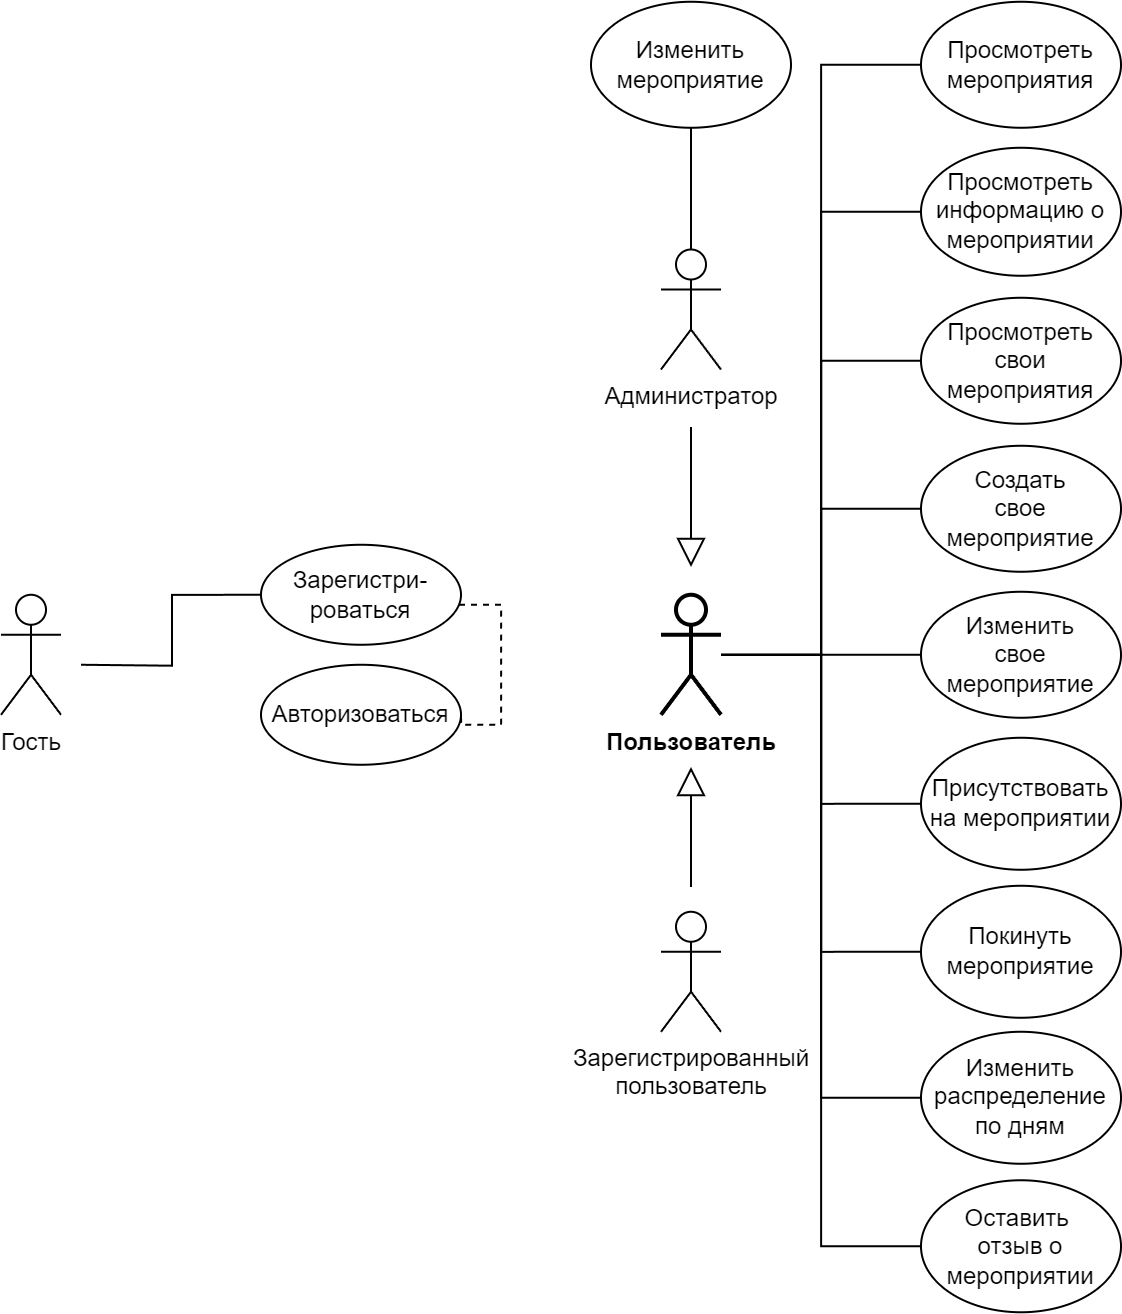
\includegraphics[width=1\textwidth]{images/use-case-2.png}
	\caption{Диаграмма прецендентов} 
	\label{fig:use-case-diagram} 
\end{figure}

\section{Описание сущностей базы данных}

На основе данных, представленных в таблице~\ref{tbl:data-groups}, можно определить таблицы, которые должны быть включены в базу данных:
\begin{enumerate}
	\item locations -- таблица локаций;
	\item events -- таблица мероприятий;
	\item persons -- таблица участников мероприятий;
	\item days -- таблица дней мероприятий;
	\item menu -- таблица меню дней мероприятий;
	\item items -- таблица предметов меню;
	\item feedbacks -- таблица отзывов участников;
	\item users -- таблица пользователей.
\end{enumerate}

На основе информации о выбранном типе базы данных и диаграммы <<сущность-связь>> на рисунке~\ref{fig:er-diagram} можно определить структуры столбцов, их типы и ограничения для каждой таблицы, которые представлены в таблицах~\ref{tbl:locations}-\ref{tbl:users}.

\begin{table}[h!]
	\centering
	\caption{Информация о таблице локаций}
	\begin{tabularx}{\textwidth}{|p{2.6cm}|X|p{6cm}|X|}
		\hline
		\textbf{Атрибут} & \textbf{Тип данных} & \textbf{Ограничения} & \textbf{Сведение} \\
		\hline
		location\_id & UUID & NOT~NULL, \newline PRIMARY~KEY & Идентификатор локации \\
		\hline
		name & Строковой & NOT~NULL & Название \\
		\hline
		description & Строковой & NOT~NULL & Описание \\
		\hline
		price & Вещественный & NOT~NULL, \newline CHECK~(price~>=~0) & Цена аренды на 1 день \\
		\hline
		capacity & Целочисленный & NOT~NULL, \newline CHECK~(capacity~>=~0) & Вместимость \\
		\hline
	\end{tabularx}
	\label{tbl:locations}
\end{table}

\begin{table}[h!]
	\centering
	\caption{Информация о таблице мероприятий}
	\begin{tabularx}{\textwidth}{|p{2.6cm}|X|p{6cm}|X|}
		\hline
		\textbf{Атрибут} & \textbf{Тип данных} & \textbf{Ограничения} & \textbf{Сведение} \\
		\hline
		event\_id & UUID & NOT~NULL, \newline PRIMARY~KEY & Идентификатор мероприятия \\
		\hline
		name & Строковой & NOT~NULL & Название \\
		\hline
		description & Строковой & NOT~NULL & Описание \\
		\hline
		date & Дата & NOT~NULL & Дата \\
		\hline
		person\_count & Целочисленный & NOT~NULL, \newline CHECK~(person\_count~>=~0) & Количество участников \\
		\hline
		days\_count & Целочисленный & NOT~NULL, \newline CHECK~(days\_count~>~0) & Количество дней \\
		\hline
		percent & Вещественный & NOT~NULL, \newline CHECK~(percent~>=~0) & Наценка на посещение в процентах \\
		\hline
		rating & Вещественный & NOT~NULL, \newline CHECK (rating~BETWEEN~0~AND~10) & Рейтинг \\
		\hline
	\end{tabularx}
	\label{tbl:events}
\end{table}

\begin{table}[h!]
	\centering
	\caption{Информация о таблице дней мероприятий}
	\begin{tabularx}{\textwidth}{|p{2.6cm}|X|p{6cm}|X|}
		\hline
		\textbf{Атрибут} & \textbf{Тип данных} & \textbf{Ограничения} & \textbf{Сведение} \\
		\hline
		day\_id & UUID & NOT~NULL, \newline PRIMARY~KEY & Идентификатор дня мероприятия \\
		\hline
		name & Строковой & NOT~NULL & Название \\
		\hline
		sequence\_ number & Целочисленный & NOT~NULL, \newline CHECK (sequence\_number~>~0) & Порядковый номер \\
		\hline
		description & Строковой & NOT~NULL & Описание \\
		\hline
		price & Вещественный & NOT~NULL, \newline CHECK~(price~>=~0) & Цена посещения \\
		\hline
	\end{tabularx}
	\label{tbl:days}
\end{table}

\begin{table}[h!]
	\centering
	\caption{Информация о таблице участников мероприятий}
	\begin{tabularx}{\textwidth}{|p{2.6cm}|X|p{6cm}|X|}
		\hline
		\textbf{Атрибут} & \textbf{Тип данных} & \textbf{Ограничения} & \textbf{Сведение} \\
		\hline
		person\_id & UUID & NOT~NULL, \newline PRIMARY~KEY & Идентификатор участника \\
		\hline
		name & Строковой & NOT~NULL & Имя \\
		\hline
		type & Перечисляемый & NOT~NULL & Тип \\
		\hline
		paid & Логический & NOT~NULL & Факт оплаты \\
		\hline
	\end{tabularx}
	\label{tbl:persons}
\end{table}

\begin{table}[h!]
	\centering
	\caption{Информация о таблице меню дней мероприятий}
	\begin{tabularx}{\textwidth}{|p{2.6cm}|X|p{6cm}|X|}
		\hline
		\textbf{Атрибут} & \textbf{Тип данных} & \textbf{Ограничения} & \textbf{Сведение} \\
		\hline
		menu\_id & UUID & NOT~NULL, \newline PRIMARY~KEY & Идентификатор меню \\
		\hline
		name & Строковой & NOT~NULL & Название \\
		\hline
		cost & Вещественный & NOT~NULL, \newline CHECK~(cost~>=~0) & Стоимость \\
		\hline
	\end{tabularx}
	\label{tbl:menu}
\end{table}

\begin{table}[h!]
	\centering
	\caption{Информация о таблице предметов меню}
	\begin{tabularx}{\textwidth}{|p{2.6cm}|X|p{6cm}|X|}
		\hline
		\textbf{Атрибут} & \textbf{Тип данных} & \textbf{Ограничения} & \textbf{Сведение} \\
		\hline
		item\_id & UUID & NOT~NULL, \newline PRIMARY~KEY & Идентификатор предмета \\
		\hline
		name & Строковой & NOT~NULL & Название \\
		\hline
		type & Перечисляемый & NOT~NULL & Тип \\
		\hline
		price & Вещественный & NOT~NULL, \newline CHECK~(price~>=~0) & Цена \\
		\hline
	\end{tabularx}
	\label{tbl:items}
\end{table}

\begin{table}[h!]
	\centering
	\caption{Информация о таблице отзывов}
	\begin{tabularx}{\textwidth}{|p{2.6cm}|X|p{6cm}|X|}
		\hline
		\textbf{Атрибут} & \textbf{Тип данных} & \textbf{Ограничения} & \textbf{Сведение} \\
		\hline
		feedback\_id & UUID & NOT~NULL, \newline PRIMARY~KEY & Идентификатор отзыва \\
		\hline
		event\_id & UUID & NOT~NULL, \newline FOREIGN~KEY & Идентификатор мероприятия \\
		\hline
		person\_id & UUID & NOT~NULL, \newline FOREIGN~KEY & Идентификатор участника \\
		\hline
		comment & Строковой & NOT~NULL & Комментарий \\
		\hline
		rating & Вещественный & NOT~NULL, \newline CHECK (rating~BETWEEN~0~AND~10) & Рейтинг \\
		\hline
	\end{tabularx}
	\label{tbl:feedbacks}
\end{table}

\begin{table}[h!]
	\centering
	\caption{Информация о таблице пользователей}
	\begin{tabularx}{\textwidth}{|p{2.6cm}|X|p{6cm}|X|}
		\hline
		\textbf{Атрибут} & \textbf{Тип данных} & \textbf{Ограничения} & \textbf{Сведение} \\
		\hline
		user\_id & UUID & NOT~NULL, \newline PRIMARY~KEY & Идентификатор пользователя \\
		\hline
		phone & Строковой & NOT~NULL & Телефон \\
		\hline
		gender & Перечисляемый & NOT~NULL & Гендер \\
		\hline
		password & Строковой & NOT~NULL & Пароль \\
		\hline
		role & Перечисляемый & NOT~NULL & Роль \\
		\hline
	\end{tabularx}
	\label{tbl:users}
\end{table}

\newpage

Диаграмма базы данных представлена на рисунке~\ref{fig:db-diagram-notypes}.

\begin{figure}[h!]
	\centering
	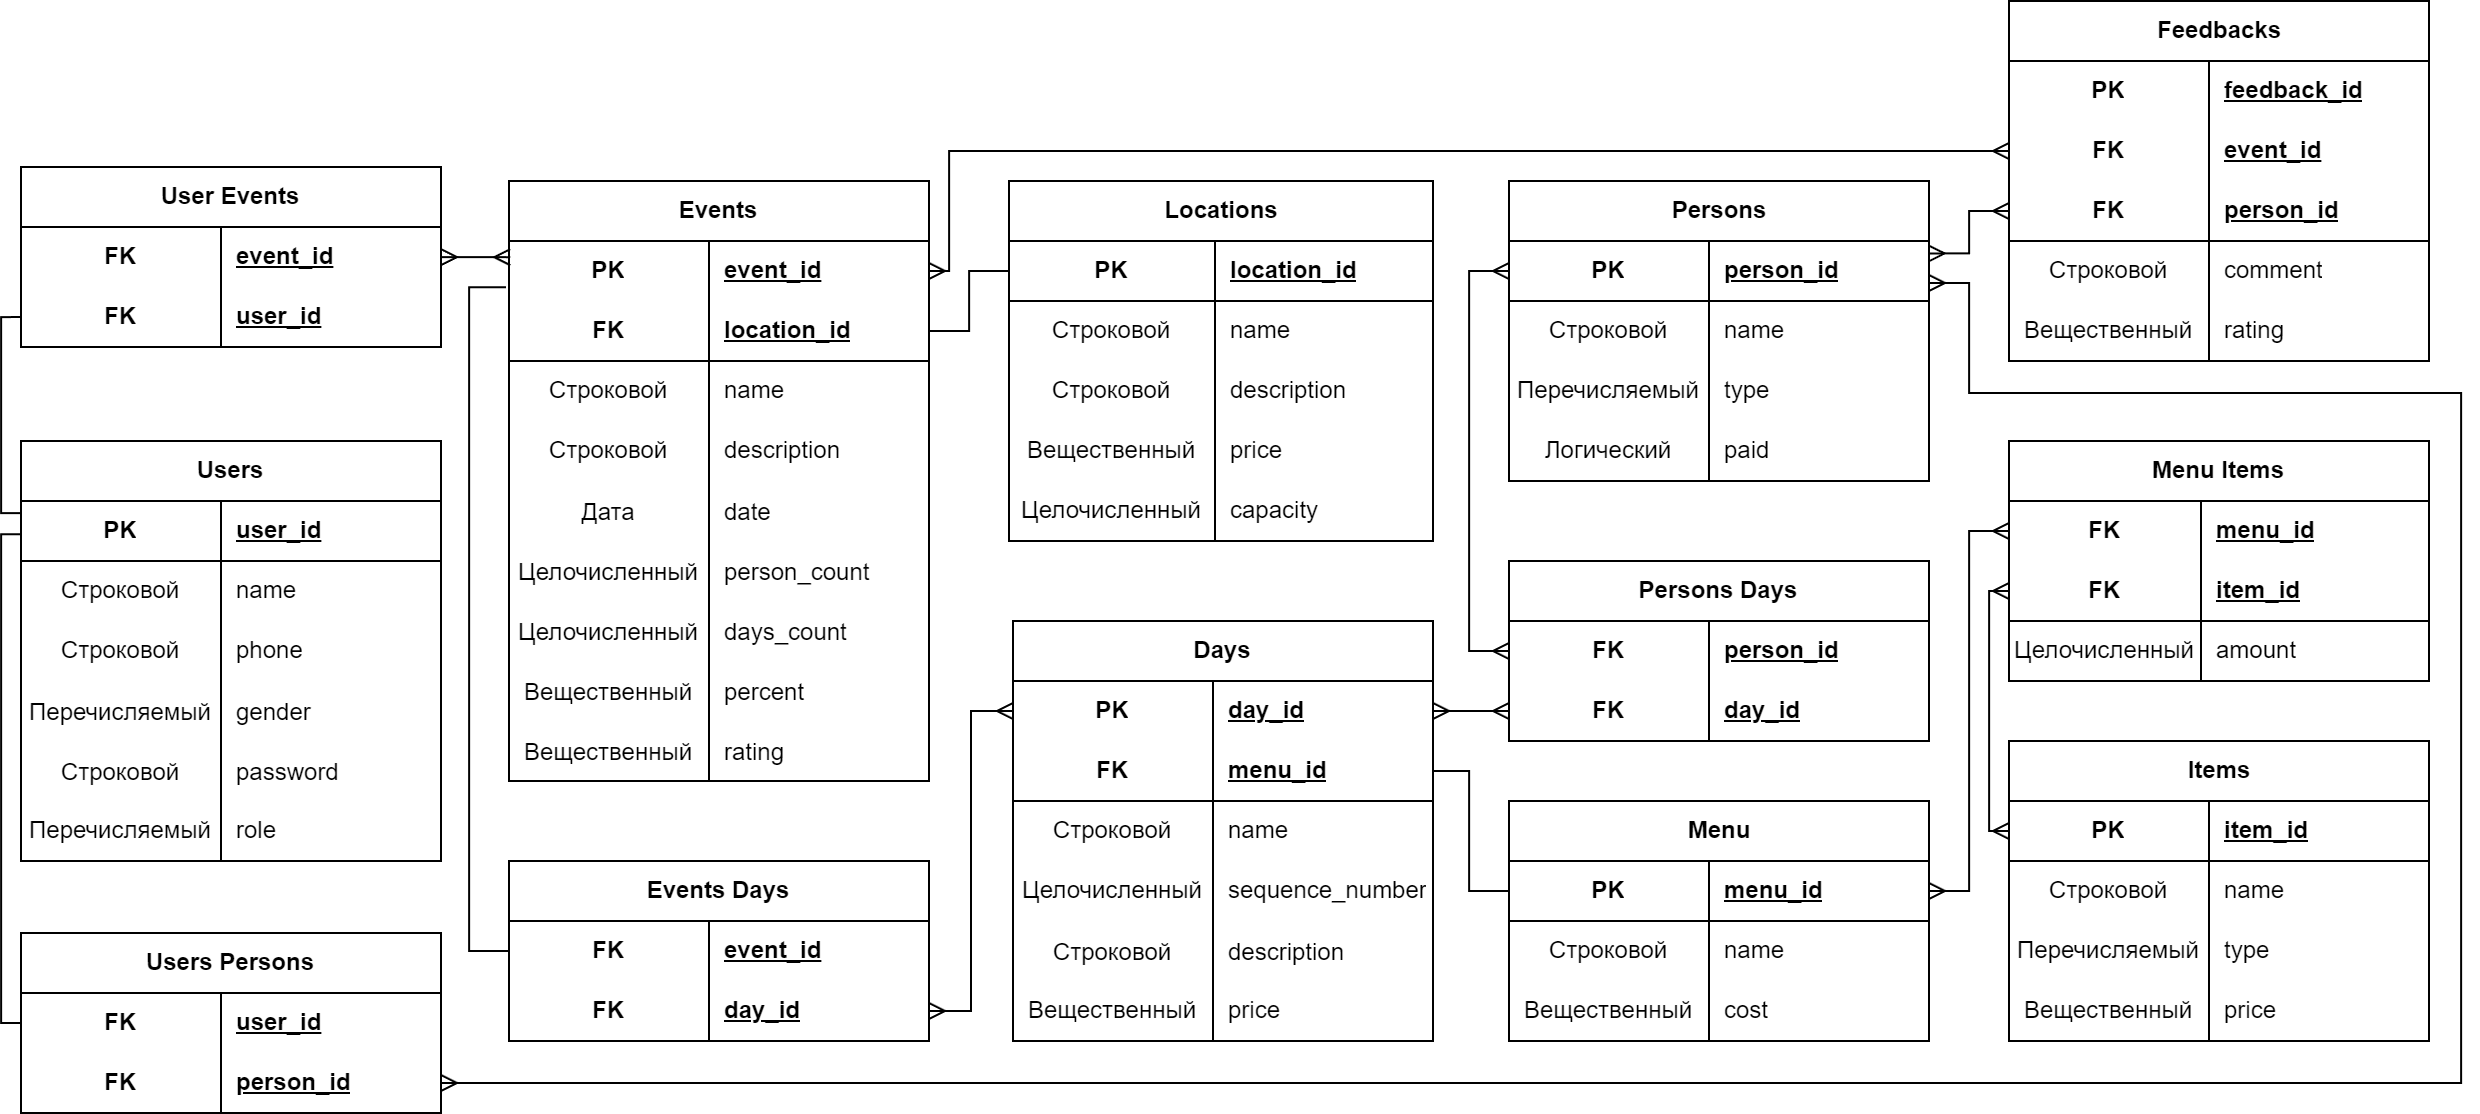
\includegraphics[width=1\textwidth]{images/db-diagram-notypes.png}
	\caption{Диаграмма базы данных} 
	\label{fig:db-diagram-notypes} 
\end{figure}

\section{Ролевая модель}

Ролевая модель в СУБД распределяет права доступа между ролями, ограничивая их действия для обеспечения безопасности:
\begin{itemize}[label=--]
	\item гость может выполнять SELECT и INSERT для таблицы пользователей;
	\item авторизованный пользователь может выполнять SELECT, INSERT, \newline UPDATE и DELETE для всех таблиц;
	\item администратор имеет все права доступа.
\end{itemize}

\section{Формализация мероприятия}

Мероприятие рассматривается как система, состоящая из участников, дней, предметов, меню и других элементов. 

\subsection{Определение мероприятия}

\textit{Множеством участников} называется группа людей, участвующих в мероприятии и обозначается:
\begin{equation}
	P = \{p_1, p_2, \dots, p_m\}
\end{equation}
где $m$ -- общее количество участников.

\textit{Множеством дней} называются временные интервалы, на которые разбито мероприятие и обозначается:
\begin{equation}
	D = \{d_1, d_2, \dots, d_n\}
\end{equation}
где $n$ -- общее количество дней.

\textit{Общим множеством предметов} называется набор материальных ресурсов необходимых для проведения и обозначается:
\begin{equation}
	O = \{o_1, o_2, \dots, o_k\}
\end{equation}
где $k$ -- общее количество предметов.

\textit{Общим множеством меню} называется множество наборов предметов  и обозначается:
\begin{equation}
	M = \{m_1, m_2, \dots, m_p\}
\end{equation}
где $\forall m_i \in M: m_i \subseteq O$ и $p$ -- общее количество меню.

\textit{Множеством меню} называется множество наборов предметов, привязанных к конкретным дням и обозначается:
\begin{equation}
	DM = \{(d, m): (d, m) \in D \times M\}
\end{equation}
где $d \in D$ -- день мероприятия, $m \in M$ -- меню, соответствующее этому дню и $\forall d \in D \ \exists! m \in M: (d, m) \in DM$.

\textit{Множеством посещений} называется множество связей участников с днями их присутствия и обозначается:
\begin{equation}
	PD = \{(p, c): (p, c) \in P \times 2^D \}
\end{equation}
где $p \in P$ -- участник, $c \in 2^D$ -- подмножество дней, которые участник $p$ планирует посетить, и $\forall p \in P \ \exists! c \in 2^D: (p, c) \in PD$.

\textit{Мероприятием} называется кортеж, объединяющий все перечисленные множества и обозначается:
\begin{equation}
	E = (P, D, O, M, PD, DM)
\end{equation}

\subsection{N-мерные случаи}

\textit{Одномерным случаем} называется ситуация выбора участником $p \in P$ ровно одного дня для посещения мероприятия, то есть:
\begin{equation}
	p \in P \ \exists! (p, c) \in PD: |c| = 1
\end{equation}

\textit{Общим одномерным случаем} называется ситуация выбора всеми участниками $p \in P$ ровно одного дня для посещения мероприятия, то есть:
\begin{equation}
	\forall p \in P \ \exists! (p, c) \in PD: |c| = 1
\end{equation}

\textit{$N$-мерным случаем} называется ситуация выбора участником $p \in P$ ровно $n$ дней для посещения мероприятия, то есть:
\begin{equation}
	p \in P \ \exists! (p, c) \in PD: |c| = n
\end{equation}

\textit{Общим $n$-мерным случаем} называется ситуация выбора всеми участниками $p \in P$ от 1-го до $n$ дней для посещения мероприятия, то есть:
\begin{equation}
	\forall p \in P \ \exists! (p, c) \in PD: |c| \in \{1, \dots, n\}
\end{equation}

Из определения следует, что общий одномерный случай является частным примером общего $n$-мерного случая.

\subsection{Базис мероприятия}

\textit{Базисом мероприятия} называется множество функций, обрабатывающих его.

Функции базиса можно классифицировать следующим образом:
\begin{enumerate}
	\item первого порядка -- функции, рассматривающие одномерный случай;
	\item $n$-го порядка -- функции, рассматривающие $n$-мерный случай.
\end{enumerate}

Из определения следует, что функции первого порядка являются частным примером функций $n$-го порядка.

\subsubsection{Функции стоимости}

\textit{Функцией стоимости C} называется функция, ставящая своему объекту-аргументу в соответствие его денежную стоимость. Областью определения функции $C$ является $D(C) = E \cup D \cup M \cup O$, а областью значений $E(C) = \mathbb{R}_{\ge 0}$.

\textit{Функция стоимости предмета} обозначается как:
\begin{equation}
	C_O: O \rightarrow \mathbb{R}_{\ge 0}
\end{equation}

\textit{Функция стоимости меню} обозначается как $C_M: M \rightarrow \mathbb{R}_{\ge 0}$ и определяется как сумма всех стоимостей предметов, входящих в меню:
\begin{equation}
	C_M(m) = \sum_{o_i \in m} C_O(o_i)
\end{equation}

\textit{Функция стоимости дня первого порядка} обозначается как \newline $C_D: D \rightarrow \mathbb{R}_{\ge 0}$ и определяется как стоимость меню, соответствующего этому дню:
\begin{equation}
	C_D(d) = C_M(m), \ \text{где} \ (d, m) \in DM
\end{equation}

\textit{Функция стоимости дня $n$-го порядка} обозначается как $C_D: D^n \rightarrow \mathbb{R}_{\ge 0}$ \newline и определяется как сумма всех стоимостей меню, соответствующих \newline набору-аргументу из $n$ дней:
\begin{equation}
	C_D(d_1, \dots, d_n) = \sum_{d_i \in (d_1, \dots, d_n)}{C_M(m)}, \ \text{где} \ (d_i, m) \in DM
\end{equation}

\textit{Функция стоимости мероприятия} обозначается как $C_E: E \rightarrow \mathbb{R}_{\ge 0}$ и определяется как сумма стоимостей всех дней мероприятия:
\begin{equation}
	C_E(E) = \sum_{d_i \in D} C_D(d_i)
	\label{eq:cost-event}
\end{equation}

\subsubsection{Функции цены}

\textit{Функцией цены P} называется функция, ставящая своему объекту-аргументу в соответствие цену его посещения участником $p \in P$. Областью определения функции $P$ является $D(P) = E \cup D$, а областью значений $E(P) = \mathbb{R}_{\ge 0}$.

\textit{Функция цены дня первого порядка} обозначается как:
\begin{equation}
	P_D: D \rightarrow \mathbb{R}_{\ge 0}
\end{equation}

\textit{Функция цены дня n-го порядка} обозначается как:
\begin{equation}
	P_D: D^n \rightarrow \mathbb{R}_{\ge 0}
\end{equation}

\textit{Функция цены мероприятия} обозначается как $P_E: E \rightarrow \mathbb{R}_{\ge 0}$ и определяется как сумма цен посещения всех его дней:
\begin{equation}
	P_E(E) = \sum_{d_i \in D}{P_D(d_i)}
\end{equation}

\subsubsection{Вспомогательные функции}

\textit{Функция текущих комбинаций дней} обозначается как $H: E \rightarrow 2^D$ и определяется как множество текущих комбинаций дней $c \in 2^D$, выбранных участниками $P$:
\begin{equation}
	H(E) = \{c: p \in P \ \exists! c: (p, c) \in PD\}
\end{equation}

\textit{Функция количества человек дня первого порядка} обозначается как \newline $N_D: D \rightarrow \mathbb{N}$ и определяется как мощность множества участников конкретного дня:
\begin{equation}
	N_D(d) = |\{p: (p, d) \in PD\}|
\end{equation}

\textit{Функция количества человек дня n-го порядка} обозначается как \newline $N_D: D^n \rightarrow \mathbb{N}$ и определяется как мощность множества участников конкретного набора из $n$ дней:
\begin{equation}
	N_D(d_1, \dots, d_n) = |\{p: (p, (d_1, \dots, d_n)) \in PD\}|
\end{equation}

\textit{Функция строгого количества человек дня первого порядка} обозначается как $N_D^*: D \rightarrow \mathbb{N}$ и определяется как мощность множества участников, посещающих только конкретный день:
\begin{equation}
	N_D^*(d) = |\{p:(p, d) \in PD \wedge \forall d_i \in D \setminus d : (p, d_i) \notin PD\}|
\end{equation}

\textit{Функция строгого количества человек дня n-го порядка} обозначается как $N_D^*: D^n \rightarrow \mathbb{N}$ и определяется как мощность множества участников, посещающих только дни конкретной комбинации:
\begin{equation}
	N_D^*(c) = |\{p:(p, c) \in PD \wedge \forall d_i \in D \setminus c : (p, d_i) \notin PD\}|
\end{equation}

\textit{Функция количества человек мероприятия} обозначается как \newline $N_E: E \rightarrow \mathbb{N}$ и определяется как мощность множества участников:
\begin{equation}
	N_E(E) = |P|
\end{equation}

\textit{Функция коэффициента дня первого порядка} обозначается как \newline $A: D \rightarrow \mathbb{R}_{\ge 0}$ и определяется как отношение стоимости дня к минимальной стоимости:
\begin{equation}
	A(d) = \frac{C_D(d)}{\min_{d_i \in D}{C_D(d_i)}}
\end{equation}

\textit{Функция коэффициента дня n-го порядка} обозначается как \newline $A: D^n \rightarrow \mathbb{R}_{\ge 0}$ и определяется как сумма отношений стоимости каждого дня из набора к минимальной стоимости:
\begin{equation}
	A(d_1, \dots, d_n) = \frac{1}{\min_{d_i \in D}{C_D(d_i)}}\sum_{d_i \in \{d_1, \dots, d_n\}}{C_D(d_i)}
\end{equation}

\subsection{Уравнения баланса}

\subsubsection{Общий одномерный случай}

Чтобы все расходы на конкретный день были покрыты, необходимо, чтобы доходы от участников этого дня были им равны:
\begin{equation}
	C_D(d) = P_D(d) \cdot N_D(d)
	\label{eq:cost-price-1}
\end{equation}

Из определения~\ref{eq:cost-event} и уравнения~\ref{eq:cost-price-1} имеем:
\begin{equation}
	C_E(E) = \sum_{d_i \in D} C_D(d_i) = \sum_{d_i \in D}{P_D(d_i) \cdot N_D(d_i)}
	\label{eq:balance-equation-1}
\end{equation}

\subsubsection{Общий n-мерный случай}

Чтобы все расходы на конкретную комбинацию дней были покрыты, необходимо, чтобы доходы от участников этой комбинации были им равны:
\begin{equation}
	C_D(d_1, \dots, d_n) = P_D(d_1, \dots, d_n) \cdot N_D^*(d_1, \dots, d_n)
	\label{eq:cost-price-2}
\end{equation}

В $n$-мерном случае участники оплачивают присутствие не на конкретных днях, а на их комбинациях, потому, чтобы покрыть расходы на всё мероприятие, необходимо покрыть расходы на все комбинации:
\begin{equation}
	C_E(E) = \sum_{c_i \in H(E)}{P_D(c_i) \cdot N_D^*(c_i)}
	\label{eq:balance-equation-2}
\end{equation}

Уравнения~\ref{eq:balance-equation-1} и~\ref{eq:balance-equation-2} называются \textit{уравнениями баланса} для общих одномерного и $n$-мерного случаев соответственно.

\subsection{Фундаментальная цена}

Фундаментальная цена -- это формальное решение уравнения баланса, которое используется для расчета цены посещения каждого дня мероприятия. Она определяется таким образом, чтобы цена каждого дня мероприятия была пропорциональна его стоимости.

Цена посещения дня выражается через фундаментальную цену $P_0$ и коэффициент дня:
\begin{itemize}[label=--]
	\item для одномерного случая:
	\begin{equation}
		P_D(d) = A(d) \cdot P_0(E)
		\label{eq:price-by-fundamental-price-1}
	\end{equation}
	\item для $n$-мерного случая:
	\begin{equation}
		P_D(d_1, \dots, d_n) = A(d_1, \dots, d_n) \cdot P_0(E)
		\label{eq:price-by-fundamental-price-2}
	\end{equation}
\end{itemize}  

В силу линейности уравнения баланса, если фундаментальная цена существует, она единственна:
\begin{equation}
	P_0 = P_0(E)
\end{equation}

\subsubsection{Общий одномерный случай}

Подставив уравнение~\ref{eq:price-by-fundamental-price-1} в уравнение~\ref{eq:cost-price-1}, имеем:
\begin{equation}
	C_D(d) = A(d) \cdot P_0 \cdot N_D(d)
	\label{eq:cost-by-fundamental-1}
\end{equation}

Подставив уравнение~\ref{eq:cost-by-fundamental-1} в уравнение баланса~\ref{eq:balance-equation-1}, имеем:
\begin{equation}
	C_E(E) = \sum_{d_i \in D}{A(d_i) \cdot P_0 \cdot N_D(d_i)} = P_0 \cdot \sum_{d_i \in D}{A(d_i) \cdot N_D(d_i)}
	\label{eq:balance-equation-by-fundamental-1}
\end{equation}

Из уравнения~\ref{eq:balance-equation-by-fundamental-1} имеем:
\begin{equation}
	P_0(E) = \frac{C_E(E)}{\sum_{d_i \in D}{A(d_i) \cdot N_D(d_i)}}
	\label{eq:fundamental-price-1}
\end{equation}

\subsubsection{Общий n-мерный случай}

Подставив уравнение~\ref{eq:price-by-fundamental-price-2} в уравнение~\ref{eq:cost-price-2}, имеем:
\begin{equation}
	C_D(d_1, \dots, d_n) = A(d_1, \dots, d_n) \cdot P_0 \cdot N_D^*(d_1, \dots, d_n)
	\label{eq:cost-by-fundamental-2}
\end{equation}

Подставив уравнение~\ref{eq:cost-by-fundamental-2} в уравнение баланса~\ref{eq:balance-equation-2}, имеем:
\begin{equation}
	C_E(E) = \sum_{c_i \in H(E)}{A(c_i) \cdot P_0 \cdot N_D^*(c_i)} = P_0 \cdot \sum_{c_i \in H(E)}{A(c_i) \cdot N_D^*(c_i)}
	\label{eq:balance-equation-by-fundamental-2}
\end{equation}

Из уравнения~\ref{eq:balance-equation-by-fundamental-2} имеем:
\begin{equation}
	P_0(E) = \frac{C_E(E)}{\sum_{c_i \in H(E)}{A(c_i) \cdot N_D^*(c_i)}}
	\label{eq:fundamental-price-2}
\end{equation}

\subsection{Получение прибыли}

Наличие прибыли -- это финансовый результат, при котором доходы от мероприятия превышают его затраты. В рамках уравнения баланса условие наличия прибыли можно обозначить как:
\begin{equation}
	C_E(E) < \sum_{c_i \in H(E)}{P_D(c_i) \cdot N_D^*(c_i)} \Leftrightarrow \sum_{c_i \in H(E)}{P_D(c_i) \cdot N_D^*(c_i)} - C_E(E) > 0
\end{equation}

Прибыль определяется как положительная разница между совокупным доходом от участников мероприятия и общими затратами на его организацию:

\begin{equation}
	\Pi = \sum_{c_i \in H(E)}{P_D(c_i) \cdot N_D^*(c_i)} - C_E(E)
\end{equation}

Прибыль может быть реализована через процентную наценку на фундаментальную цену. Пусть $\alpha \ge 0$ -- коэффициент, увеличивающий фундаментальную цену $P_0$. Тогда функция цены посещения конкретного дня примет вид:
\begin{equation}
	P_D'(c_i) = (1 + \alpha) \cdot A(c_i) \cdot P_0
\end{equation}

Прибыль в этом случае будет равна:
\begin{equation}
	\Pi = \sum_{c_i \in H(E)}{P_D'(c_i) \cdot N_D^*(c_i)} - C_E(E) 
\end{equation}
\begin{equation}
	\Pi = (1 + \alpha) \cdot \sum_{c_i \in H(E)}{P_D(c_i) \cdot N_D^*(c_i)} - C_E(E)
\end{equation}
\begin{equation}
	\Pi = (1 + \alpha) \cdot C_E(E) - C_E(E) = \alpha \cdot C_E(E)
\end{equation}

\subsection{Известные теоремы}

\subsubsection{Теорема об условии существования решения}

Уравнение баланса для общего $n$-мерного случая имеет решение, только если:
\begin{equation}
	\begin{cases}
		\forall d \in D: C_D(d) > 0 \\
		\forall d \in D: N_D(d) > 0
	\end{cases}
\end{equation}

\textit{Доказательство:} для существования решения уравнения баланса необходимо и достаточно: a) чтобы существовала фундаментальная цена; б) чтобы были покрыты все затраты на мероприятие. 

а) из формулы~\ref{eq:fundamental-price-2} имеем, что для существования фундаментальной цены требуется:
\begin{equation}
	\sum_{c_i \in H(E)}{A(c_i) \cdot N_D(c_i)} > 0
	\label{eq:exist-cond}
\end{equation}

Условие~\ref{eq:exist-cond} не выполняется, если:
\begin{itemize}[label=--]
	\item $\exists c_i \in H(E): A(c_i) \ \text{не определено, то есть} \ \min_{d_i \in D}{C_D(d_i)} = 0$;
	\item $\exists c_i \in H(E): N_D(c_i) = 0, \text{то есть} \ H(E) = \emptyset \Leftrightarrow PD = \emptyset$.
\end{itemize}

Следовательно, для выполнения условия~\ref{eq:exist-cond} необходимо и достаточно:
\begin{equation}
	\begin{cases}
		\forall d \in D: C_D(d) > 0 \\
		PD \ne \emptyset
	\end{cases}
	\label{eq:a_system}
\end{equation}

б) если $\exists d \in D: N_D(d) = 0$, то затраты на этот день в случае их наличия не покрываются, так как $P_D(d) \cdot N_D(d) = 0$. Следовательно, фундаментальная цена $P_0$ не является решением уравнения баланса. Значит, для покрытия затрат на всё мероприятие необходимо следующее условие:
\begin{equation}
	\forall d \in D: C_D(d) > 0 \Rightarrow N_D(d) > 0
	\label{eq:n(d)>0}
\end{equation}

Добавив условие~\ref{eq:n(d)>0} в систему~\ref{eq:a_system}, имеем:
\begin{equation}
	\begin{cases}
		\forall d \in D: C_D(d) > 0 \\
		PD \ne \emptyset \\
		\forall d \in D: C_D(d) > 0 \Rightarrow N_D(d) > 0
	\end{cases} 
	=
	\begin{cases}
		\forall d \in D: C_D(d) > 0 \\
		PD \ne \emptyset \\
		\forall d \in D: N_D(d) > 0
	\end{cases}
\end{equation}

Заметив, что $\forall d \in D: N_D(d) > 0 \Rightarrow PD \ne \emptyset$, в итоге имеем:
\begin{equation}
	\begin{cases}
		\forall d \in D: C_D(d) > 0 \\
		\forall d \in D: N_D(d) > 0
	\end{cases}
\end{equation}

\subsubsection{Теорема об инвариантности к масштабу}

Если все стоимости $C_D(d)$ возрастут в $k$ раз, то фундаментальная цена $P_0$ так же возрастет в $k$ раз, при этом:
\begin{equation}
	\frac{P_D(d)}{P_D'(d)} = \frac{1}{k}
\end{equation}
где $P_D'(d)$ -- изменённая функция цены.

\textit{Доказательство:} пусть $C_D'(d) = k \cdot C_D(d)$, тогда:
\begin{itemize}[label=--]
	\item $A'(d) = \frac{C_D'(d)}{\min_{d_i \in D}{C_D'(d_i)}} = \frac{k \cdot C_D(d)}{k \cdot \min_{d_i \in D}{C_D(d)}} = A(d)$;
	\item $C_E'(E) = \sum_{d_i \in D}{C_D'(d_i)} = k \cdot \sum_{d_i \in D}{C_D(d_i)} = k \cdot C_E(E)$.
\end{itemize}

Следовательно, имеем:
\begin{equation}
	P_0' = \frac{C_E'(E)}{\sum_{c_i \in H(E)}{A'(c_i) \cdot N_D(c_i)}} = \frac{k \cdot C_E(E)}{\sum_{c_i \in H(E)}{A(c_i) \cdot N_D(c_i)}} = k \cdot P_0
\end{equation}

При этом $P_D'(d) = A'(d) \cdot P_0' = A(d) \cdot k \cdot P_0 = k \cdot P_D(d)$, то есть:
\begin{equation}
	\frac{P_D(d)}{P_D'(d)} = \frac{1}{k}
\end{equation}

\subsubsection{Теорема о равномерном распределении}

При общем одномерном случае, если участники распределены по дням равномерно и все их стоимости одинаковы, то и цены их посещения равны.

\textit{Доказательство:} по условию имеем
\begin{equation}
	\forall d \in D:
	\begin{cases}
		N_D(d) = N \\
		C_D(d) = C
	\end{cases}
\end{equation}

Следовательно:
\begin{equation}
	\forall d \in D: A(d) = \frac{C_D(d)}{min_{d_i \in D}{C_D(d_i)}} = \frac{C}{C} = 1
\end{equation}

Тогда при условии $|D| = n$:
\begin{equation}
	P_0 = \frac{C_E(E)}{\sum_{d_i \in D}{A(d_i) \cdot N_D(d_i)}} = \frac{n \cdot C}{\sum_{d_i \in D}{N_D(d_i)}} = \frac{n \cdot C}{n \cdot N} = \frac{C}{N}
\end{equation}

Имеем:
\begin{equation}
	\forall d \in D: P_D(d) = A(d) \cdot P_0 = 1 \cdot \frac{C}{N} = \frac{C}{N}
\end{equation}

\subsubsection{Теорема о количестве участников}

Мощность множества участников равна сумме количеств участников каждой текущей комбинации:
\begin{equation}
	|P| = \sum_{c_i \in H(E)}{N_D(c_i)}
\end{equation}

\textit{Доказательство:} из определения $PD$ следует, что каждый участник $p \in P$ выбирает ровно одну комбинацию дней $c \subseteq D$. То есть:
\begin{equation}
	\forall p \in P \ \exists! c \in H(E): (p, c) \in PD
\end{equation}

Множество участников $P$ можно разбить на непересекающиеся множества $P_{c_i}$, где каждое $P_{c_i}$ содержит участников, выбравших комбинацию $c_i$:
\begin{equation}
	P = \bigcup_{c_i \in H(E)}{P_{c_i}}, \text{где} \ P_{c_i} = \{p: (p, c_i) \in PD\}
\end{equation}

Поскольку все $P_{c_i}$ попарно не пересекаются, то мощность их объединения равна сумме их мощности:
\begin{equation}
	|P| = \sum_{c_i \in H(E)}{|P_{c_i}|}
\end{equation}

Из определения имеем $N_D(c_i) = |P_{c_i}|$. Следовательно:
\begin{equation}
	|P| = \sum_{c_i \in H(E)}{N_D(c_i)}
\end{equation}

\subsubsection{Теорема о критическом количестве участников}

Для покрытия расходов мероприятия с стоимостью $C_E(E)$ и максимальной ценой посещения $P_{max}$ необходимо:
\begin{equation}
	|P| \ge \frac{C_E(E)}{P_{max}}
\end{equation}

\textit{Доказательство:} из условия имеем:
\begin{equation}
	P_{max} = max_{c_i \in H(E)}{P_D(c_i)}
\end{equation}

Рассмотрим уравнение баланса:
\begin{equation}
	C_E(E) = \sum_{c_i \in H(E)}{P_D(c_i) \cdot N_D(c_i)} \le max_{c_i \in H(E)}{P_D(c_i)} \cdot \sum_{c_i \in H(E)}{N_D(c_i)}
	\label{ineq:cost-event}
\end{equation}

Применив теорему о количестве участников, неравенство~\ref{ineq:cost-event} можно переписать следующим образом:
\begin{equation}
	C_E(E) \le P_{max} \cdot |P| \Leftrightarrow |P| \ge \frac{C_E(E)}{P_{max}}
\end{equation}

\subsubsection{Теорема об ограничении наценки}

Коэффициент наценки $\alpha$ при условии $P_D(c_i) \le P_{max}$ для всех комбинаций дней $c_i \in H(E)$ ограничен сверху:
\begin{equation}
	\alpha \le \min_{c_i \in H(E)}{\Big(\frac{P_{max}}{A(c_i) \cdot P_0} - 1\Big)}
\end{equation}

\textit{Доказательство:} по определению цены комбинации дней с наценкой:
\begin{equation}
	P_D(c_i) = (1 + \alpha) \cdot A(c_i) \cdot P_0
\end{equation}

Условие $\forall c_i \in H(E): P_D(c_i) \le P_{max}$ может быть записано следующим образом:
\begin{equation}
	(1 + \alpha) \cdot A(c_i) \cdot P_0 \le P_{max} \Leftrightarrow \alpha \le \frac{P_{max}}{A(c_i) \cdot P_0} - 1
\end{equation}

Чтобы неравенство выполнялось для всех $c_i$, выберем минимальное значение правой части:
\begin{equation}
	\alpha \le \min_{c_i \in H(E)}{\Big(\frac{P_{max}}{A(c_i) \cdot P_0} - 1\Big)}
\end{equation}

\subsubsection{Теорема о самом дешевом дне}

Если участники концентрируются на дне с минимальной стоимостью $C_D(d)$, то фундаментальная цена $P_0$ возрастает.

\textit{Доказательство:} пусть $d' \in D$ -- день с минимальной стоимостью, то есть $C_D(d') = \min_{d_i \in D}{C_D(d_i)}$. Тогда имеем по определению коэффициента дня:
\begin{equation}
	A(d') = \frac{C_D(d')}{\min_{d_i \in D}{C_D(d_i)}} = \frac{\min_{d_i \in D}{C_D(d_i)}}{\min_{d_i \in D}{C_D(d_i)}} = 1
\end{equation}

Если $N_D(d')$ увеличивается при $N_E(E) = const$, тогда существует день \newline $d \in D, d \ne d'$ такой, что $N_D(d)$ уменьшается. Следовательно, \newline $\sum_{c_i \in H(E)}{A(c_i) \cdot N_D(c_i)}$ будет уменьшаться, так как $\forall d \in D: A(d') \le A(d)$, и $P_0$ будет возрастать.

\section{Используемые триггеры}

В базе данных реализованы следующие триггеры, каждый из которых автоматизирует управление связанными данными мероприятий, включая создание и удаление связанных сущностей, синхронизацию количества дней, обновление количества участников, динамическое ценообразование, пересчёт стоимости меню и рейтинга мероприятия:
\begin{enumerate}
	\item Триггер создания связанных данных мероприятия --  автоматически создаёт связанные дни и меню при добавлении нового мероприятия;
	\item Триггер синхронизации количества дней -- поддерживает актуальное количество дней мероприятия при изменении связей, увеличивает или уменьшает число дней в соответствии с заданным значением, удаляя или добавляя необходимые сущности;
	\item Триггер обновления количества участников -- пересчитывает общее число участников мероприятия при изменении данных о посещении дней, учитывает добавление, удаление или изменение записей о присутствии;
	\item Триггер динамического ценообразования -- автоматически корректирует цены дней при изменении влияющих параметров;
	\item Триггер удаления связанных данных -- обеспечивает каскадное удаление всех связанных сущностей при удалении мероприятия, гарантируя целостность данных;
	\item Триггер обновления стоимости меню -- пересчитывает стоимость меню при изменении его состава;
	\item Триггер расчёта рейтинга мероприятия -- обновляет средний рейтинг мероприятия при добавлении, изменении или удалении отзывов.
\end{enumerate}

\section{Архитектура приложения}

Структура данного приложения основана на принципах чистой архитектуры. Данная архитектура направлена на создание систем, которые легко модифицировать и тестировать, а также которые обеспечивают высокую степень независимости от внешних факторов, таких как фреймворки, базы данных и пользовательские интерфейсы~\cite{lit10}.

\begin{figure}[h]
	\centering
	\includegraphics[width=0.7\textwidth]{images/clean-architecture.png}
	\caption{Слои приложения согласно принципам чистой архитектуры} 
	\label{fig:clean-architecture} 
\end{figure}

В рамках этой архитектуры приложение структурировано таким образом, что бизнес-логика отделена от деталей реализации, что позволяет сосредоточиться на функциональности без необходимости беспокоиться о том, как именно функции будут реализованы в различных средах. Это достигается за счёт четкого разделения на уровни, где каждый уровень отвечает за свою область ответственности~\cite{lit10}.

\subsection{Диаграмма потока данных}

Поток данных в приложении инициируется взаимодействием пользователя с графическим интерфейсом, передающим действия в контроллеры слоя представления. Контроллеры перенаправляют запросы в слой бизнес-логики, где данные проходят валидацию и обработку в соответствии с установленными правилами. Бизнес-логика взаимодействует с адаптерами для выполнения операций с базой данных, после чего обработанные данные возвращаются через слои приложения в графический интерфейс для отображения.

Диаграмма потока данных представлена на рисунке~\ref{fig:data-flow}.

\begin{figure}[h]
	\centering
	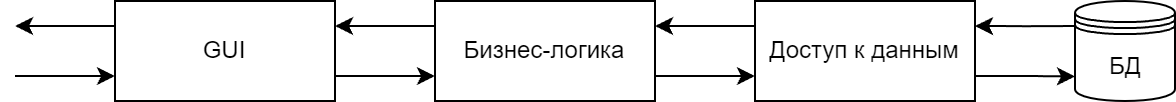
\includegraphics[width=1\textwidth]{images/data-flow.png}
	\caption{Диаграмма потока данных} 
	\label{fig:data-flow} 
\end{figure}

\subsection{Диаграмма компонентов}

Диаграмма компонентов представлена на рисунке~\ref{fig:components-diagram}.

\begin{figure}[h]
	\centering
	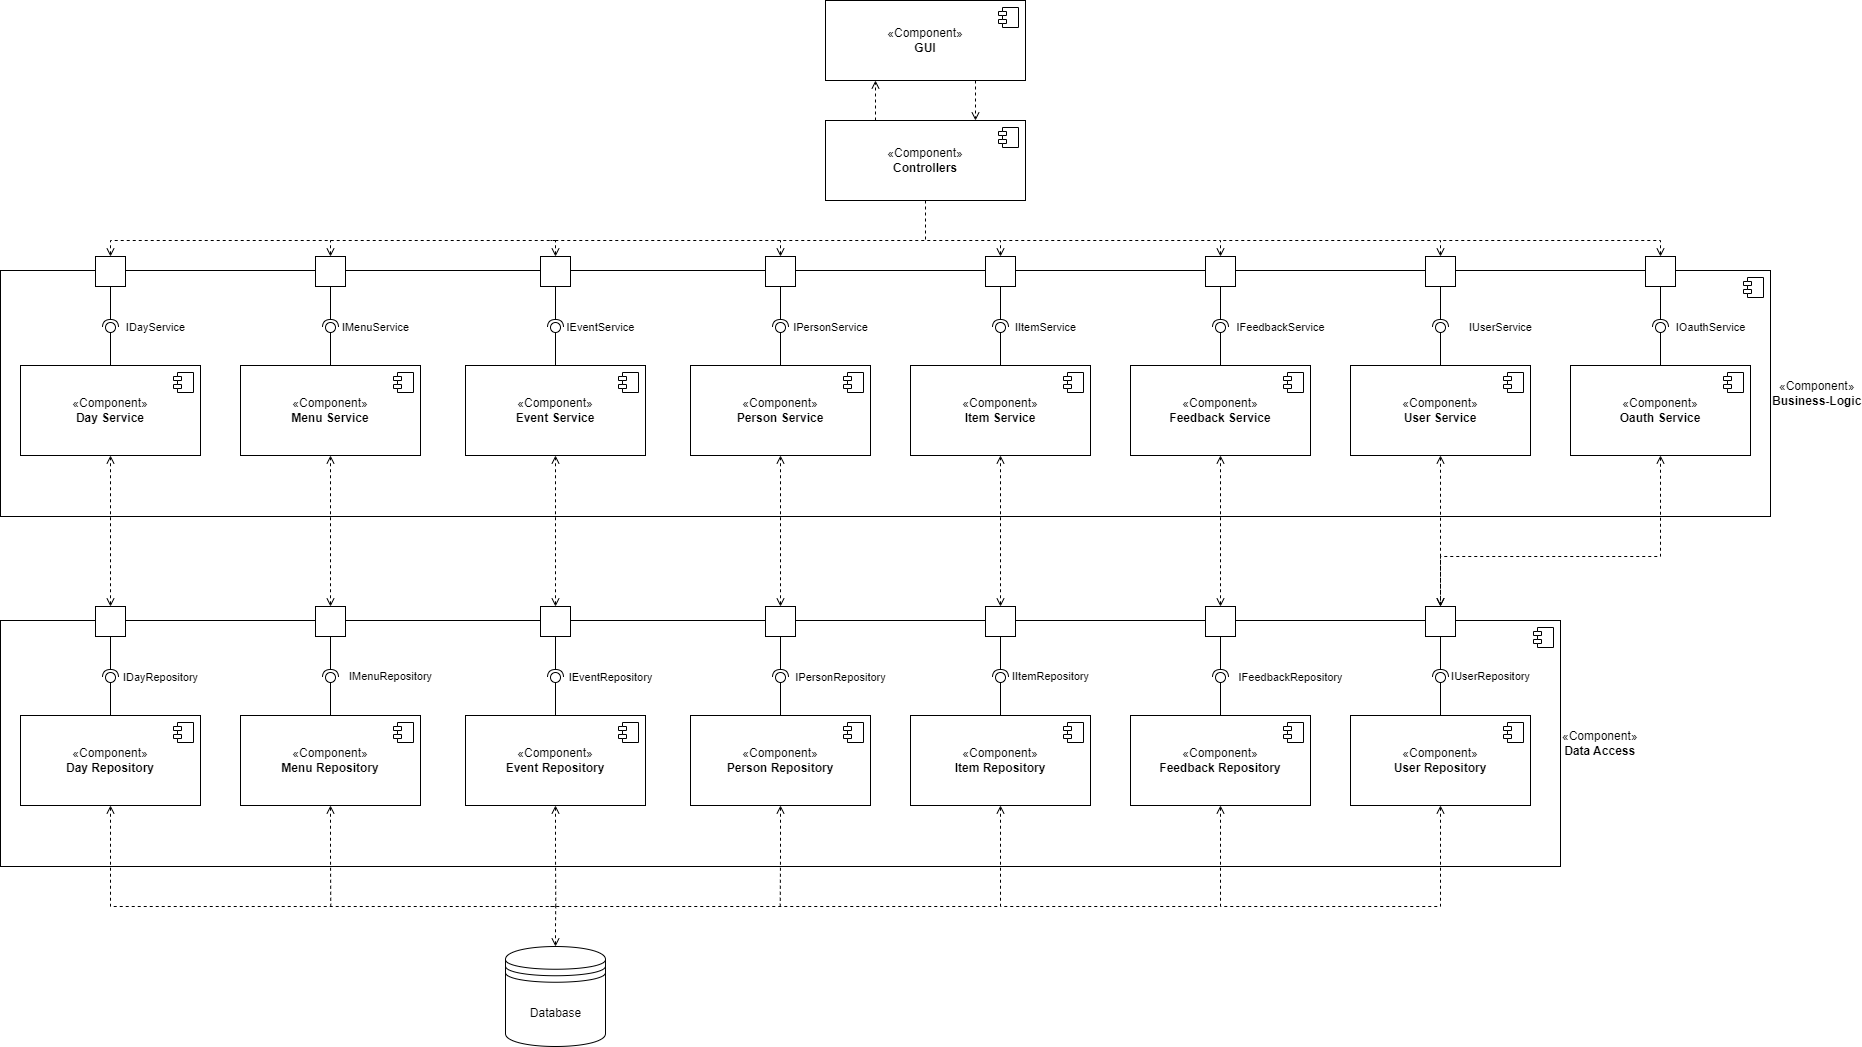
\includegraphics[width=1\textwidth]{images/uml-components.png}
	\caption{Диаграмма компонентов} 
	\label{fig:components-diagram} 
\end{figure}


\subsection{Диаграмма классов}

Диаграмма классов представлена на рисунке~\ref{fig:class-diagram}.

\begin{figure}[h]
	\centering
	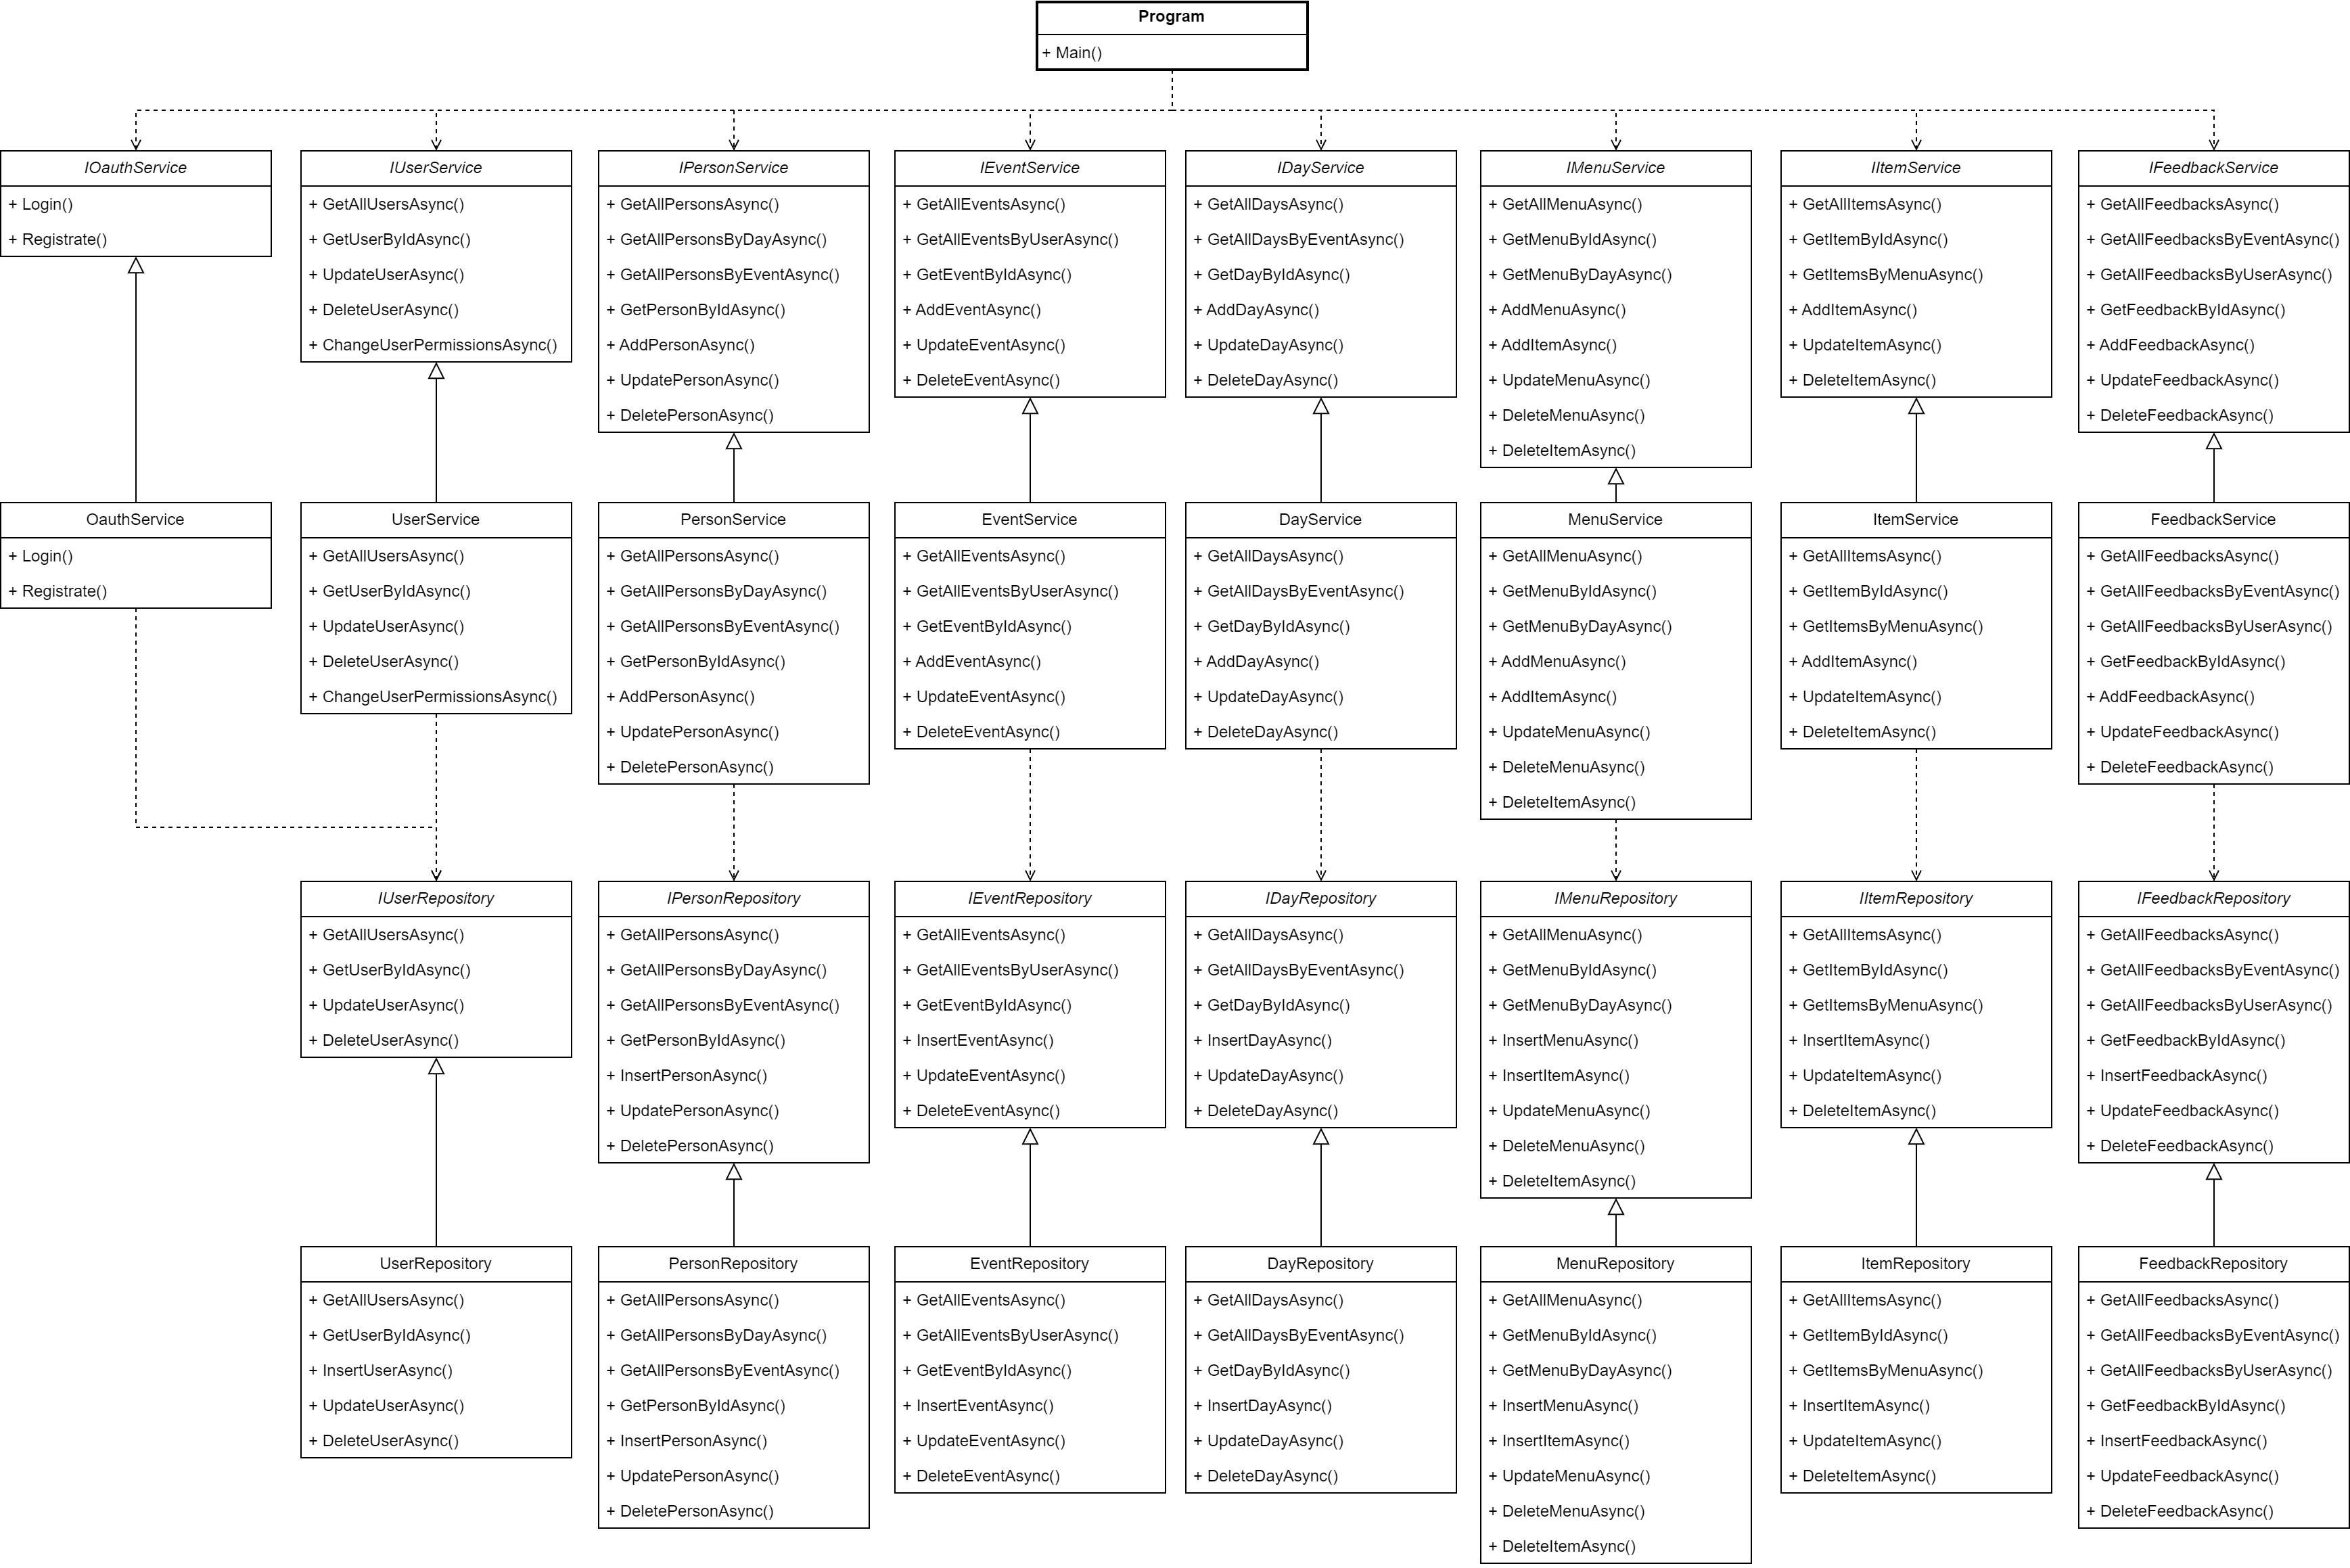
\includegraphics[width=1\textwidth]{images/uml-classes.png}
	\caption{Диаграмма классов} 
	\label{fig:class-diagram} 
\end{figure}

\section{Вывод}

В конструкторской части работы были сформулированы требования к программе, разработаны диаграммы прецедентов и базы данных, определены структуры таблиц с типами данных и ограничениями, формализована модель мероприятия, описаны триггеры для автоматизации процессов, а также представлена архитектура приложения с диаграммами потоков данных, компонентов и классов.

\clearpage
